\documentclass[10pt]{standalone}
\usepackage{tikz}
\usetikzlibrary{
  calc,
  patterns,
  decorations.pathmorphing,
}





\begin{document}

\noindent

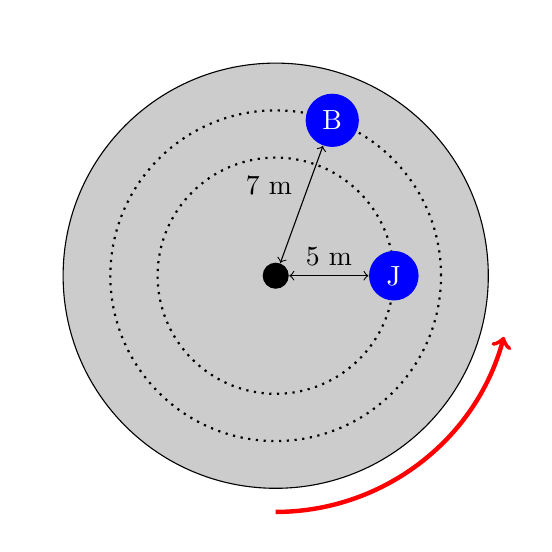
\begin{tikzpicture}[x=3mm,y=3mm]
  \clip (-10.5,-10.5) rectangle (10.5,10.5);
  \draw[fill=gray!40] (0,0) circle (9);
  \node[circle,minimum size=0.5,fill=black] 
    at (0,0) (center) {};
  \draw[dotted,thick] (0,0) circle (5);
  \draw[dotted,thick] (0,0) circle (7);
  \node[circle,white,fill=blue] at (0:5)
    (Janey) {J};
  \node[circle,white,fill=blue] at (70:7)
    (Bobby) {B};
  \draw[<->] (center) -- (Janey) 
    node[midway,above] {5 m};
  \draw[<->] (center) -- (Bobby) 
    node[midway,above left] {7 m};

  \draw[->,ultra thick,red] (-90:10) arc (-90:-15:10);
\end{tikzpicture}



\end{document}